\documentclass[12pt]{article}
\usepackage{graphicx} % For including images
\usepackage[margin=1in]{geometry} % For setting page margins
\usepackage{amsmath} % For extended mathematical formatting
\usepackage{fancyhdr} % For custom headers and footers
\usepackage{float} 
\usepackage{subcaption} % Updated to use subcaption instead of subfigure
\setlength{\headheight}{15pt} % Adjust headheight as recommended
\pagestyle{fancy}
\fancyhf{}
\rhead{EE569 Digital Image Processing}
\lhead{HOMEWORK \#5}
\rfoot{Page \thepage}
\usepackage{enumitem}
\setlist[itemize]{font=\bfseries} 
\begin{document}
	
	\begin{center}
		\Large
		\textbf{Homework \#6}
		
		\vspace{0.2cm}
		\normalsize
		Issued: 03/28/2024 \hfill Due: 05/01/2024
	\end{center}
\section*{Problem 1: Origin of Green Learning (GL)}
\subsection*{(a) Feedforward-designed Convolutional Neural Networks (FF-CNNs)}
	\begin{figure}[H]
		\centering
		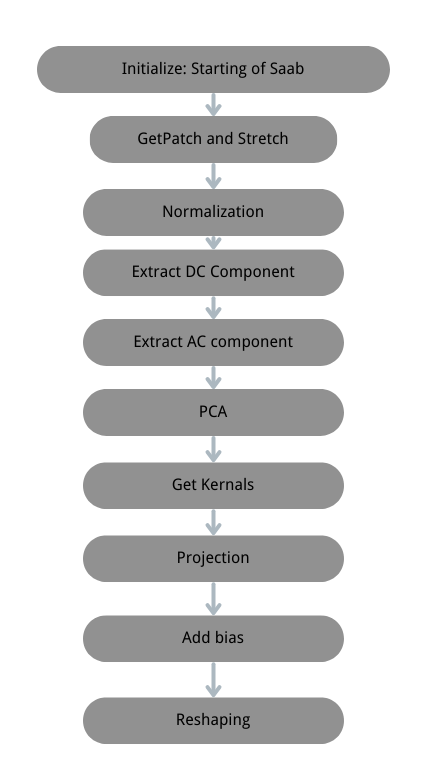
\includegraphics[width=0.6\textwidth]{saab.jpg}



	\caption{CIFAR-10 trainings}
	\label{p2b}
\end{figure}
\end{document}